\documentclass[]{article}
\usepackage{lmodern}
\usepackage{amssymb,amsmath}
\usepackage{ifxetex,ifluatex}
\usepackage{fixltx2e} % provides \textsubscript
\ifnum 0\ifxetex 1\fi\ifluatex 1\fi=0 % if pdftex
  \usepackage[T1]{fontenc}
  \usepackage[utf8]{inputenc}
\else % if luatex or xelatex
  \ifxetex
    \usepackage{mathspec}
    \usepackage{xltxtra,xunicode}
  \else
    \usepackage{fontspec}
  \fi
  \defaultfontfeatures{Mapping=tex-text,Scale=MatchLowercase}
  \newcommand{\euro}{€}
\fi
% use upquote if available, for straight quotes in verbatim environments
\IfFileExists{upquote.sty}{\usepackage{upquote}}{}
% use microtype if available
\IfFileExists{microtype.sty}{%
\usepackage{microtype}
\UseMicrotypeSet[protrusion]{basicmath} % disable protrusion for tt fonts
}{}
\usepackage[margin=1in]{geometry}
\ifxetex
  \usepackage[setpagesize=false, % page size defined by xetex
              unicode=false, % unicode breaks when used with xetex
              xetex]{hyperref}
\else
  \usepackage[unicode=true]{hyperref}
\fi
\hypersetup{breaklinks=true,
            bookmarks=true,
            pdfauthor={FEDORU},
            pdftitle={Enquête logiciels SU - Septembre 2015},
            colorlinks=true,
            citecolor=blue,
            urlcolor=blue,
            linkcolor=magenta,
            pdfborder={0 0 0}}
\urlstyle{same}  % don't use monospace font for urls
\usepackage{graphicx,grffile}
\makeatletter
\def\maxwidth{\ifdim\Gin@nat@width>\linewidth\linewidth\else\Gin@nat@width\fi}
\def\maxheight{\ifdim\Gin@nat@height>\textheight\textheight\else\Gin@nat@height\fi}
\makeatother
% Scale images if necessary, so that they will not overflow the page
% margins by default, and it is still possible to overwrite the defaults
% using explicit options in \includegraphics[width, height, ...]{}
\setkeys{Gin}{width=\maxwidth,height=\maxheight,keepaspectratio}
\setlength{\parindent}{0pt}
\setlength{\parskip}{6pt plus 2pt minus 1pt}
\setlength{\emergencystretch}{3em}  % prevent overfull lines
\providecommand{\tightlist}{%
  \setlength{\itemsep}{0pt}\setlength{\parskip}{0pt}}
\setcounter{secnumdepth}{5}

%%% Use protect on footnotes to avoid problems with footnotes in titles
\let\rmarkdownfootnote\footnote%
\def\footnote{\protect\rmarkdownfootnote}

%%% Change title format to be more compact
\usepackage{titling}

% Create subtitle command for use in maketitle
\newcommand{\subtitle}[1]{
  \posttitle{
    \begin{center}\large#1\end{center}
    }
}

\setlength{\droptitle}{-2em}
  \title{Enquête logiciels SU - Septembre 2015}
  \pretitle{\vspace{\droptitle}\centering\huge}
  \posttitle{\par}
  \author{FEDORU}
  \preauthor{\centering\large\emph}
  \postauthor{\par}
  \predate{\centering\large\emph}
  \postdate{\par}
  \date{07/09/2015}


% Redefines (sub)paragraphs to behave more like sections
\ifx\paragraph\undefined\else
\let\oldparagraph\paragraph
\renewcommand{\paragraph}[1]{\oldparagraph{#1}\mbox{}}
\fi
\ifx\subparagraph\undefined\else
\let\oldsubparagraph\subparagraph
\renewcommand{\subparagraph}[1]{\oldsubparagraph{#1}\mbox{}}
\fi

\begin{document}
\maketitle

{
\hypersetup{linkcolor=black}
\setcounter{tocdepth}{2}
\tableofcontents
}
\section{7/9/2015}\label{section}

Reprise de l'exploitation des logiciels des SU

\begin{itemize}
\tightlist
\item
  fichier source: DATA/FEDORU - ENQUETE LOGICIEL 2015 - V2 (12 06 15)
  (3)
\item
  création d'un dossier spécifique \textbf{Septembre2015} contenent un
  sous dossier \textbf{data} pour y stocker les résultats régionaux sous
  forme de fichier .csv.
\end{itemize}

\subsection{17/9/2015}\label{section-1}

\begin{itemize}
\tightlist
\item
  récup données ORUMIP (Olivier Azema)
\end{itemize}

\subsection{Récupération des fichiers
csv}\label{recuperation-des-fichiers-csv}

\begin{itemize}
\tightlist
\item
  les 5 premières lignes sont éliminées
\item
  élimination du héader =\textgreater{} il faudre en créer un
\end{itemize}

\begin{verbatim}
path = "./data/" # ./Septembre2015/data/ si console
out.file <- NULL
file.names <- dir(path, pattern =".csv") # seuls les fichiers se terminant par csv sont lus
for(i in 1:length(file.names)){
   file <- read.table(paste(path, file.names[i], sep=""), skip = 5, header = FALSE, sep=",", stringsAsFactors=FALSE)
   # on ne garde que les 22 premières colonnes
   file <- file[, 1:22]
   # on ne garde que les lignes où les colonnes 1 à 5 ne sont pas vides (http://genometoolbox.blogspot.fr/2014/01/remove-rows-with-na-values-from-r-data.html)
   file <- file[complete.cases(file[,1:5]),]
   # remplacement de la virgule écimale par le point décimal (soirce: http://stackoverflow.com/questions/5487164/r-how-to-replace-parts-of-variable-strings-within-data-frame)
   file <- as.data.frame(sapply(file, gsub, pattern = ",", replacement = "."))

   out.file <- rbind(out.file, file)
 }

n <- c("Region", "Departement", "FINESS", "Hopital", "CP", "Routage","Logiciel_2014","Editeur", "RPU_transmis","Nb_RPU_T1_2015", "Logiciel_2015", "Version_2015", "Coment", "Freq_remontee", "DN_exhaus","DN_confor", "DP_exhaus", "DP_confor", "MS_exhaus", "MS_confor", "Jours_manquants", "coment2")
 names(out.file) <- n

write.table(out.file, file = "archive.csv", sep=",", row.names = FALSE, qmethod = "double", fileEncoding="utf-8")
\end{verbatim}

\subsection{Récupération du fichier des
données}\label{recuperation-du-fichier-des-donnees}

\begin{itemize}
\tightlist
\item
  Nombre de régions participantes: 8
\item
  Nombre de sites: 224
\end{itemize}

\section{Cartographie}\label{cartographie}

Cartographie des régions participantes et des logiciels.

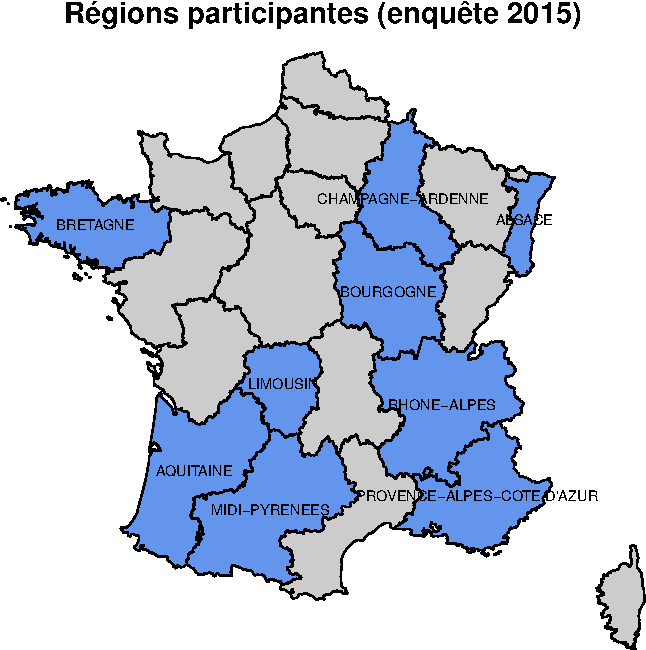
\includegraphics{septembre2015_files/figure-latex/carto_region-1.pdf}

\section{Editeurs}\label{editeurs}

\section{Logiciels 2015}\label{logiciels-2015}

\begin{itemize}
\tightlist
\item
  Nombre de logiciels utilisés: 43
\end{itemize}

\subsection{Logiciels par ordre
décroissant}\label{logiciels-par-ordre-decroissant}

\begin{verbatim}

            TU-ORUPACA                 URQUAL            RESURGENCES 
                    45                     36                     27 
                   DMU       SILLAGE URGENCES                 DXCARE 
                    14                     14                     13 
              CROSSWAY               ATALANTE                  SIDSU 
                    12                      9                      9 
             POLYMEDIS              MEDIBOARD                  ORUV2 
                     5                      4                      4 
           SILLAGE DMU          DOPA URGENCES               DOPASOIN 
                     4                      3                      3 
                 ORBIS ANTARES V2 DE INOVACUM               CLINICOM 
                     3                      2                      2 
              CORTEXTE        HOPITAL MANAGER         MÉDICAL OBJECT 
                     2                      2                      2 
                 MEDIS                  OSOFT             RPUEXPRESS 
                     2                      2                      2 
               SANOCOM              SHAREGATE                 SIGEMS 
                     2                      2                      2 
           AGFA EXAGON                AXIGATE  DEVELOPPEMENT INTERNE 
                     1                      1                      1 
                DIAMMS                    DPU                   EMED 
                     1                      1                      1 
          EXPERT SANTÉ                 M-PLUS                 MANUEL 
                     1                      1                      1 
              MEDIBASE               MEDINTUX                 NAFAMA 
                     1                      1                      1 
                OSIRIS                  QCARE                SPEC 4D 
                     1                      1                      1 
            TRACK CARE 
                     1 
\end{verbatim}

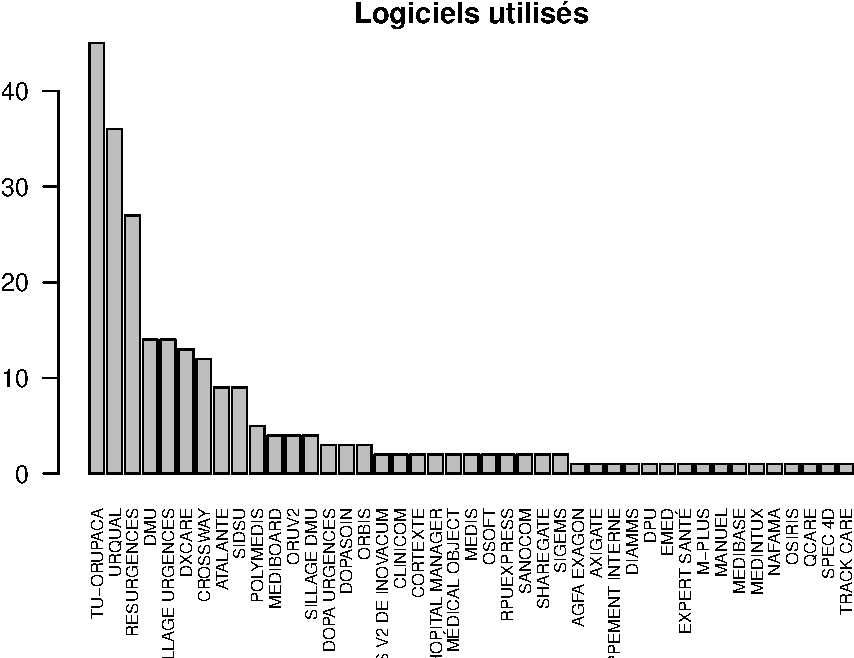
\includegraphics{septembre2015_files/figure-latex/unnamed-chunk-4-1.pdf}

\subsection{Logiciels par région}\label{logiciels-par-region}

\begin{verbatim}
                        
                         ALSACE AQUITAINE BOURGOGNE BRETAGNE
  AGFA EXAGON                 0         0         1        0
  ANTARES V2 DE INOVACUM      2         0         0        0
  ATALANTE                    8         0         1        0
  AXIGATE                     0         1         0        0
  CLINICOM                    1         0         0        0
  CORTEXTE                    0         0         0        0
  CROSSWAY                    0         3         3        0
  DEVELOPPEMENT INTERNE       0         0         0        0
  DIAMMS                      0         0         0        0
  DMU                         2         0         7        0
  DOPA URGENCES               0         1         0        0
  DOPASOIN                    0         0         0        0
  DPU                         0         0         0        0
  DXCARE                      3         6         1        0
  EMED                        0         0         0        0
  EXPERT SANTÉ                0         0         0        0
  HOPITAL MANAGER             0         0         2        0
  M-PLUS                      0         1         0        0
  MANUEL                      0         0         1        0
  MEDIBASE                    0         1         0        0
  MEDIBOARD                   0         0         0        2
  MÉDICAL OBJECT              0         0         0        0
  MEDINTUX                    0         0         0        0
  MEDIS                       0         0         0        2
  NAFAMA                      0         0         0        0
  ORBIS                       1         0         0        2
  ORUV2                       0         0         0        0
  OSIRIS                      0         0         0        0
  OSOFT                       0         0         0        2
  POLYMEDIS                   0         0         0        0
  QCARE                       0         0         0        0
  RESURGENCES                 1         1         3       13
  RPUEXPRESS                  0         0         0        0
  SANOCOM                     0         2         0        0
  SHAREGATE                   0         2         0        0
  SIDSU                       0         9         0        0
  SIGEMS                      0         2         0        0
  SILLAGE DMU                 0         0         0        4
  SILLAGE URGENCES            0         2         0       12
  SPEC 4D                     0         0         0        0
  TRACK CARE                  0         1         0        0
  TU-ORUPACA                  0         0         1        0
  URQUAL                      0         3         3       18
                        
                         CHAMPAGNE ARDENNES LIMOUSIN MIDI PYRENEES PACA
  AGFA EXAGON                             0        0             0    0
  ANTARES V2 DE INOVACUM                  0        0             0    0
  ATALANTE                                0        0             0    0
  AXIGATE                                 0        0             0    0
  CLINICOM                                0        0             1    0
  CORTEXTE                                0        0             2    0
  CROSSWAY                                0        0             6    0
  DEVELOPPEMENT INTERNE                   0        0             1    0
  DIAMMS                                  0        0             1    0
  DMU                                     3        0             0    2
  DOPA URGENCES                           2        0             0    0
  DOPASOIN                                0        0             3    0
  DPU                                     0        0             1    0
  DXCARE                                  1        0             2    0
  EMED                                    0        0             1    0
  EXPERT SANTÉ                            0        0             1    0
  HOPITAL MANAGER                         0        0             0    0
  M-PLUS                                  0        0             0    0
  MANUEL                                  0        0             0    0
  MEDIBASE                                0        0             0    0
  MEDIBOARD                               0        0             2    0
  MÉDICAL OBJECT                          0        0             2    0
  MEDINTUX                                0        0             0    1
  MEDIS                                   0        0             0    0
  NAFAMA                                  1        0             0    0
  ORBIS                                   0        0             0    0
  ORUV2                                   0        0             4    0
  OSIRIS                                  0        0             1    0
  OSOFT                                   0        0             0    0
  POLYMEDIS                               5        0             0    0
  QCARE                                   0        0             0    1
  RESURGENCES                             1        6             0    2
  RPUEXPRESS                              0        0             2    0
  SANOCOM                                 0        0             0    0
  SHAREGATE                               0        0             0    0
  SIDSU                                   0        0             0    0
  SIGEMS                                  0        0             0    0
  SILLAGE DMU                             0        0             0    0
  SILLAGE URGENCES                        0        0             0    0
  SPEC 4D                                 0        1             0    0
  TRACK CARE                              0        0             0    0
  TU-ORUPACA                              0        0             2   42
  URQUAL                                  3        2             5    2
\end{verbatim}

Nombre de logiciels différents par région

\begin{verbatim}
            ALSACE          AQUITAINE          BOURGOGNE 
                 7                 14                 10 
          BRETAGNE CHAMPAGNE ARDENNES           LIMOUSIN 
                 8                  7                  3 
     MIDI PYRENEES               PACA 
                17                  6 
\end{verbatim}

\subsection{Cartographie des
logiciels}\label{cartographie-des-logiciels}

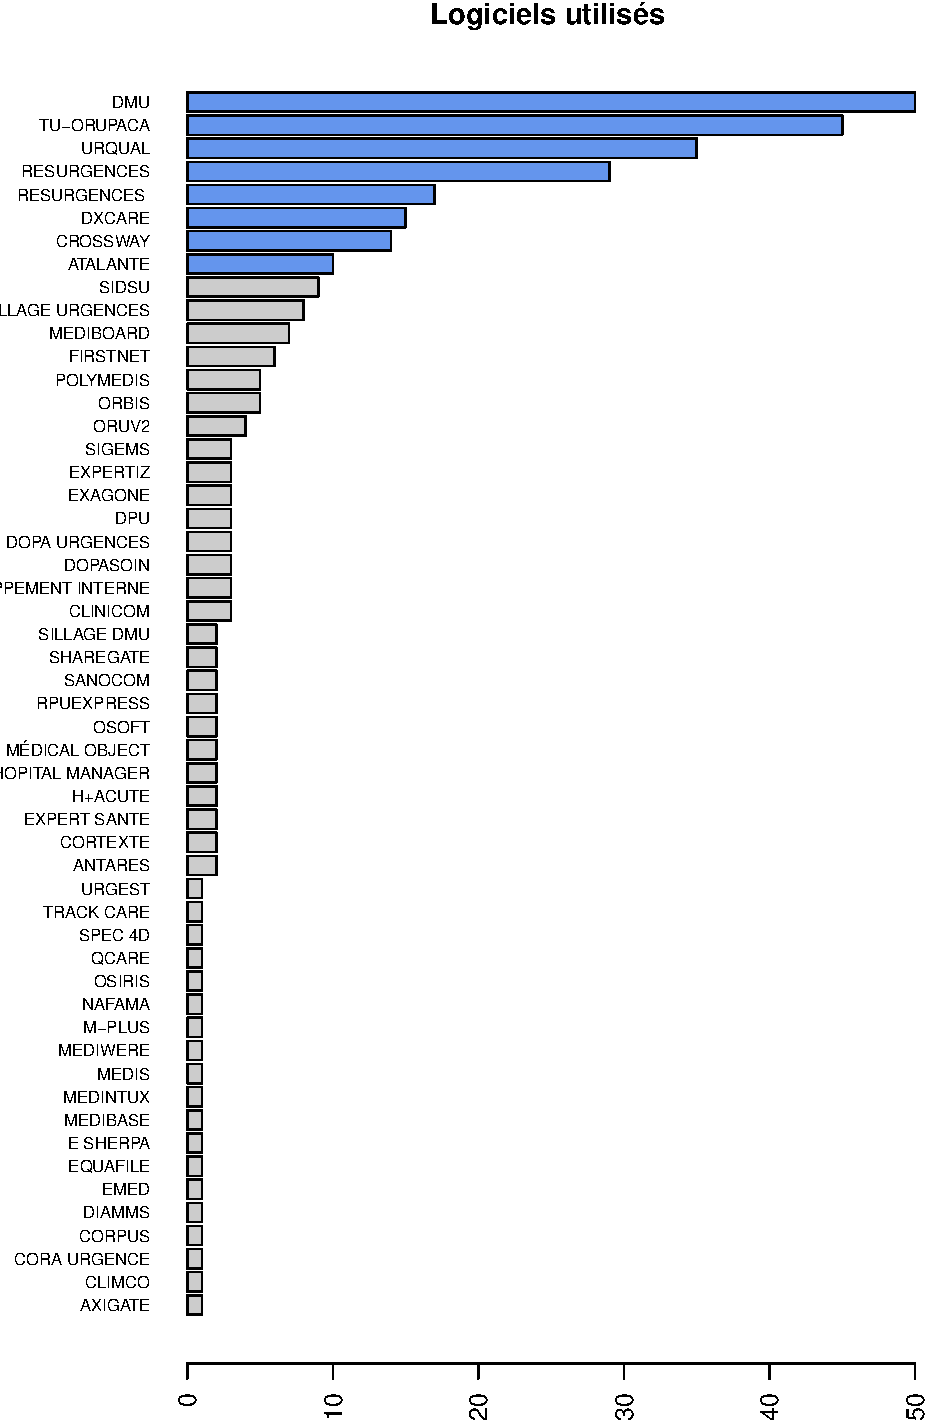
\includegraphics{septembre2015_files/figure-latex/unnamed-chunk-7-1.pdf}
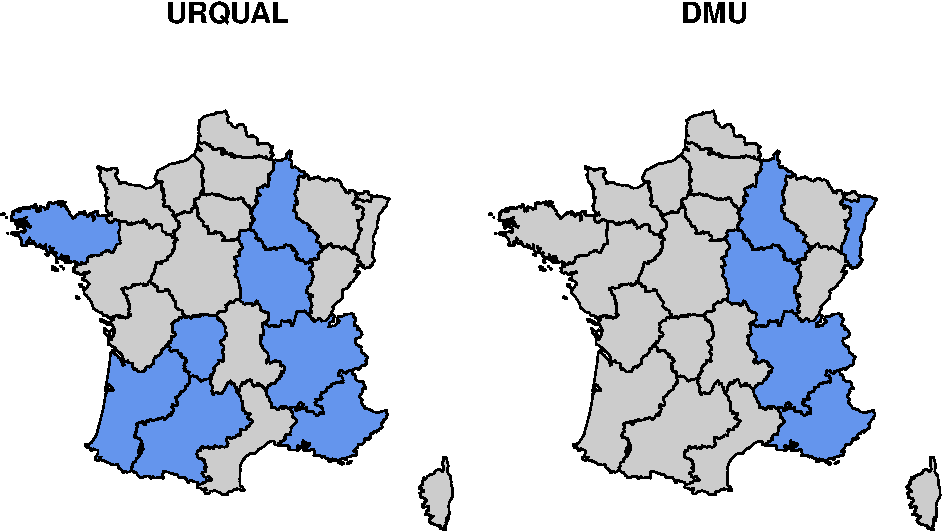
\includegraphics{septembre2015_files/figure-latex/unnamed-chunk-7-2.pdf}
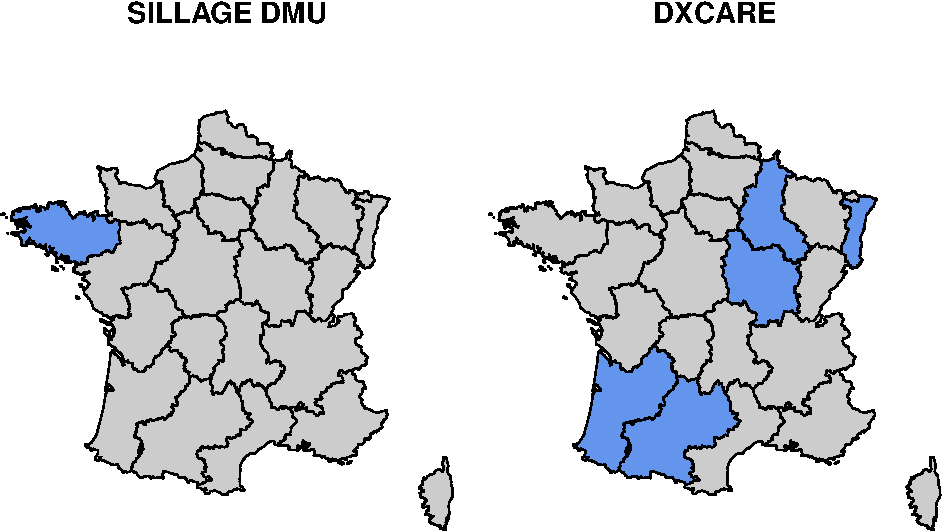
\includegraphics{septembre2015_files/figure-latex/unnamed-chunk-7-3.pdf}
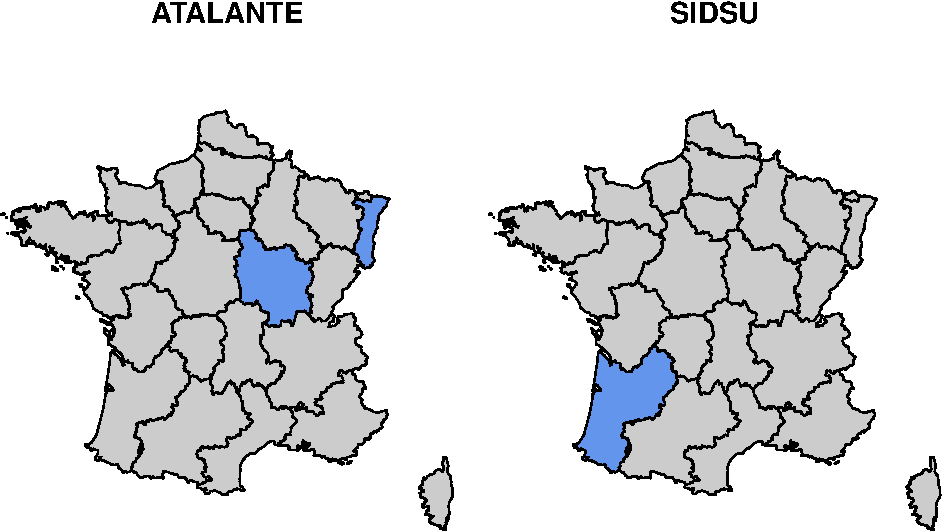
\includegraphics{septembre2015_files/figure-latex/unnamed-chunk-7-4.pdf}

\subsection{Un logiciel est présent dans combien de régions
?}\label{un-logiciel-est-present-dans-combien-de-regions}

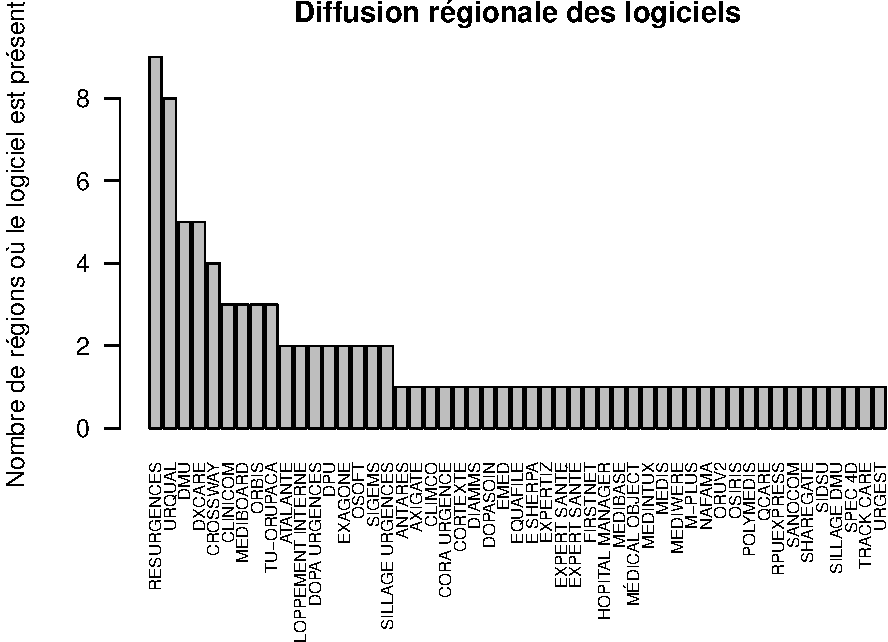
\includegraphics{septembre2015_files/figure-latex/unnamed-chunk-8-1.pdf}

\section{Analyse des RPU}\label{analyse-des-rpu}

Nombre de RPU produits: 1620416

\subsection{Nombre de RPU par
logiciel}\label{nombre-de-rpu-par-logiciel}

\begin{verbatim}
                       Nb de RPU
URQUAL                    370184
TU-ORUPACA                362364
RESURGENCES               227566
DXCARE                     97207
DMU                        80896
CROSSWAY                   60207
SILLAGE URGENCES           58588
ATALANTE                   44712
SIDSU                      44401
SILLAGE DMU                23602
MEDIBOARD                  22580
POLYMEDIS                  20363
MEDIS                      13948
MÉDICAL OBJECT             12577
CORTEXTE                   12369
TRACK CARE                 11345
ORUV2                      10715
DOPA URGENCES              10420
M-PLUS                      9970
CLINICOM                    9565
ORBIS                       9383
DOPASOIN                    9329
ANTARES V2 DE INOVACUM      8974
SHAREGATE                   8639
SANOCOM                     7150
EXPERT SANTÉ                7058
SPEC 4D                     7015
OSOFT                       6808
MEDINTUX                    6224
DPU                         5373
RPUEXPRESS                  5205
NAFAMA                      5156
QCARE                       5131
AXIGATE                     4282
SIGEMS                      3266
MEDIBASE                    2913
HOPITAL MANAGER             2644
AGFA EXAGON                 2541
MANUEL                      2504
OSIRIS                      2019
DIAMMS                      1833
DEVELOPPEMENT INTERNE       1767
EMED                        1623
\end{verbatim}

\subsection{Nombre de jours manquants}\label{nombre-de-jours-manquants}

\subsubsection{Par logiciel}\label{par-logiciel}

\begin{verbatim}
                       Nb de jours manquants
URQUAL                                   117
TU-ORUPACA                                90
SILLAGE URGENCES                          84
CROSSWAY                                  63
DOPASOIN                                  59
EMED                                      50
ORBIS                                     35
RESURGENCES                                5
CLINICOM                                   4
HOPITAL MANAGER                            3
ATALANTE                                   2
DMU                                        2
ANTARES V2 DE INOVACUM                     1
MEDIBOARD                                  1
AGFA EXAGON                                0
AXIGATE                                    0
CORTEXTE                                   0
DEVELOPPEMENT INTERNE                      0
DIAMMS                                     0
DOPA URGENCES                              0
DPU                                        0
DXCARE                                     0
EXPERT SANTÉ                               0
M-PLUS                                     0
MANUEL                                     0
MEDIBASE                                   0
MÉDICAL OBJECT                             0
MEDINTUX                                   0
MEDIS                                      0
NAFAMA                                     0
ORUV2                                      0
OSIRIS                                     0
OSOFT                                      0
POLYMEDIS                                  0
QCARE                                      0
RPUEXPRESS                                 0
SANOCOM                                    0
SHAREGATE                                  0
SIDSU                                      0
SIGEMS                                     0
SILLAGE DMU                                0
SPEC 4D                                    0
TRACK CARE                                 0
\end{verbatim}

\subsubsection{Par région}\label{par-region}

\begin{verbatim}
                   Nb de jours manquants
PACA                                 180
MIDI PYRENEES                        111
BRETAGNE                             104
AQUITAINE                             63
ALSACE                                34
BOURGOGNE                             21
CHAMPAGNE ARDENNES                     3
LIMOUSIN                               0
\end{verbatim}

\section{Indicateurs}\label{indicateurs}

Trois indicateurs ont été retenus:

\begin{itemize}
\tightlist
\item
  Date de naissance
\item
  Diagnostic principal (DP)
\item
  Mode de sortie
\end{itemize}

Chaque indicateur a été évalué sur deux critères: \textbf{conformité} et
\textbf{exhaustivité}.

\subsection{Date de naissance}\label{date-de-naissance}

\begin{itemize}
\tightlist
\item
  taux de conformité:
\end{itemize}

\begin{verbatim}
   Min. 1st Qu.  Median    Mean 3rd Qu.    Max.    NA's 
   0.00  100.00  100.00   99.57  100.00  100.00       5 
\end{verbatim}

\begin{itemize}
\tightlist
\item
  conformité par outil:
\end{itemize}

\begin{verbatim}
                          Min    Max   moyenne   ecart-type Nb
AGFA EXAGON            100.00 100.00 100.00000           NA  1
ANTARES V2 DE INOVACUM 100.00 100.00 100.00000  0.000000000  2
ATALANTE               100.00 100.00 100.00000  0.000000000  9
AXIGATE                100.00 100.00 100.00000           NA  1
CLINICOM               100.00 100.00 100.00000  0.000000000  2
CORTEXTE               100.00 100.00 100.00000  0.000000000  2
CROSSWAY                99.98 100.00  99.99727  0.006466698 12
DEVELOPPEMENT INTERNE   99.94  99.94  99.94000           NA  1
DIAMMS                 100.00 100.00 100.00000           NA  1
DMU                    100.00 100.00 100.00000  0.000000000 14
DOPA URGENCES          100.00 100.00 100.00000  0.000000000  3
DOPASOIN                99.96 100.00  99.97333  0.023094011  3
DPU                    100.00 100.00 100.00000           NA  1
DXCARE                 100.00 100.00 100.00000  0.000000000 13
EMED                   100.00 100.00 100.00000           NA  1
EXPERT SANTÉ           100.00 100.00 100.00000           NA  1
HOPITAL MANAGER        100.00 100.00 100.00000  0.000000000  2
M-PLUS                 100.00 100.00 100.00000           NA  1
MANUEL                 100.00 100.00 100.00000           NA  1
MEDIBASE               100.00 100.00 100.00000           NA  1
MEDIBOARD               99.98 100.00  99.99500  0.010000000  4
MÉDICAL OBJECT         100.00 100.00 100.00000  0.000000000  2
MEDINTUX                99.92  99.92  99.92000           NA  1
MEDIS                  100.00 100.00 100.00000  0.000000000  2
NAFAMA                  99.80  99.80  99.80000           NA  1
ORBIS                  100.00 100.00 100.00000  0.000000000  3
ORUV2                   98.74 100.00  99.64750  0.607144958  4
OSIRIS                  99.90  99.90  99.90000           NA  1
OSOFT                  100.00 100.00 100.00000  0.000000000  2
POLYMEDIS              100.00 100.00 100.00000  0.000000000  5
QCARE                   99.98  99.98  99.98000           NA  1
RESURGENCES             99.95 100.00  99.99769  0.009922779 27
RPUEXPRESS              99.89 100.00  99.94500  0.077781746  2
SANOCOM                100.00 100.00 100.00000  0.000000000  2
SHAREGATE              100.00 100.00 100.00000  0.000000000  2
SIDSU                  100.00 100.00 100.00000  0.000000000  9
SIGEMS                 100.00 100.00 100.00000           NA  2
SILLAGE DMU            100.00 100.00 100.00000  0.000000000  4
SILLAGE URGENCES       100.00 100.00 100.00000  0.000000000 14
SPEC 4D                100.00 100.00 100.00000           NA  1
TRACK CARE             100.00 100.00 100.00000           NA  1
TU-ORUPACA               0.00 100.00  97.77778 14.907119850 45
URQUAL                  99.80 100.00  99.98529  0.047688083 36
\end{verbatim}

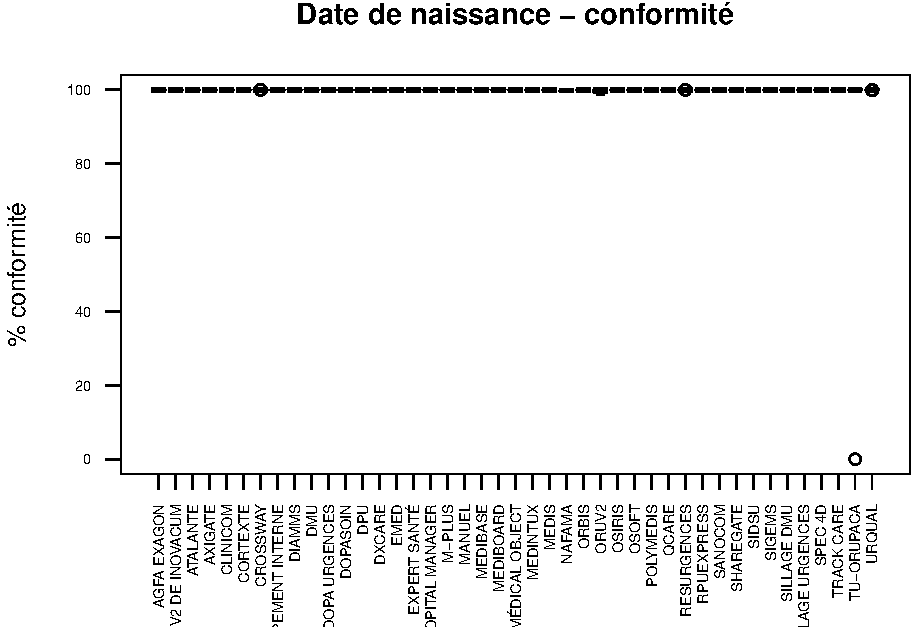
\includegraphics{septembre2015_files/figure-latex/unnamed-chunk-14-1.pdf}

\begin{itemize}
\tightlist
\item
  taux d'exhaustivité:
\end{itemize}

\begin{verbatim}
   Min. 1st Qu.  Median    Mean 3rd Qu.    Max.    NA's 
   0.00  100.00  100.00   99.58  100.00  100.00       5 
\end{verbatim}

\begin{itemize}
\tightlist
\item
  exhaustivité par outil
\end{itemize}

\begin{verbatim}
                          Min    Max   moyenne   ecart-type Nb
AGFA EXAGON            100.00 100.00 100.00000           NA  1
ANTARES V2 DE INOVACUM 100.00 100.00 100.00000  0.000000000  2
ATALANTE               100.00 100.00 100.00000  0.000000000  9
AXIGATE                100.00 100.00 100.00000           NA  1
CLINICOM               100.00 100.00 100.00000  0.000000000  2
CORTEXTE               100.00 100.00 100.00000  0.000000000  2
CROSSWAY               100.00 100.00 100.00000  0.000000000 12
DEVELOPPEMENT INTERNE  100.00 100.00 100.00000           NA  1
DIAMMS                 100.00 100.00 100.00000           NA  1
DMU                    100.00 100.00 100.00000  0.000000000 14
DOPA URGENCES          100.00 100.00 100.00000  0.000000000  3
DOPASOIN                99.96 100.00  99.97333  0.023094011  3
DPU                    100.00 100.00 100.00000           NA  1
DXCARE                 100.00 100.00 100.00000  0.000000000 13
EMED                   100.00 100.00 100.00000           NA  1
EXPERT SANTÉ           100.00 100.00 100.00000           NA  1
HOPITAL MANAGER        100.00 100.00 100.00000  0.000000000  2
M-PLUS                 100.00 100.00 100.00000           NA  1
MANUEL                 100.00 100.00 100.00000           NA  1
MEDIBASE               100.00 100.00 100.00000           NA  1
MEDIBOARD              100.00 100.00 100.00000  0.000000000  4
MÉDICAL OBJECT         100.00 100.00 100.00000  0.000000000  2
MEDINTUX                99.92  99.92  99.92000           NA  1
MEDIS                  100.00 100.00 100.00000  0.000000000  2
NAFAMA                  99.80  99.80  99.80000           NA  1
ORBIS                  100.00 100.00 100.00000  0.000000000  3
ORUV2                   99.97 100.00  99.99250  0.015000000  4
OSIRIS                 100.00 100.00 100.00000           NA  1
OSOFT                  100.00 100.00 100.00000  0.000000000  2
POLYMEDIS              100.00 100.00 100.00000  0.000000000  5
QCARE                   99.98  99.98  99.98000           NA  1
RESURGENCES             99.95 100.00  99.99769  0.009922779 27
RPUEXPRESS             100.00 100.00 100.00000  0.000000000  2
SANOCOM                100.00 100.00 100.00000  0.000000000  2
SHAREGATE              100.00 100.00 100.00000  0.000000000  2
SIDSU                  100.00 100.00 100.00000  0.000000000  9
SIGEMS                 100.00 100.00 100.00000           NA  2
SILLAGE DMU            100.00 100.00 100.00000  0.000000000  4
SILLAGE URGENCES       100.00 100.00 100.00000  0.000000000 14
SPEC 4D                100.00 100.00 100.00000           NA  1
TRACK CARE             100.00 100.00 100.00000           NA  1
TU-ORUPACA               0.00 100.00  97.77778 14.907119850 45
URQUAL                  99.99 100.00  99.99971  0.001714986 36
\end{verbatim}

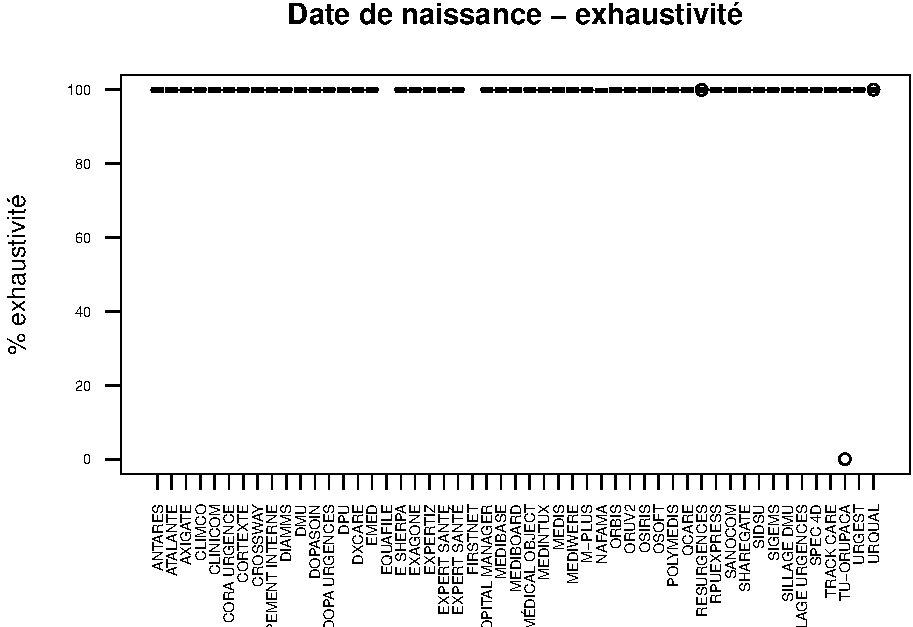
\includegraphics{septembre2015_files/figure-latex/unnamed-chunk-16-1.pdf}

\subsection{Diagnostic (DP)}\label{diagnostic-dp}

\begin{itemize}
\tightlist
\item
  taux de conformité:
\end{itemize}

\begin{verbatim}
   Min. 1st Qu.  Median    Mean 3rd Qu.    Max.    NA's 
   0.00   37.00   92.40   69.98   98.24  100.00       6 
\end{verbatim}

\begin{itemize}
\tightlist
\item
  conformité par outil
\end{itemize}

\begin{verbatim}
                          Min    Max   moyenne  ecart-type Nb
AGFA EXAGON             12.00  12.00  12.00000          NA  1
ANTARES V2 DE INOVACUM  45.84  90.51  68.17500 31.58645992  2
ATALANTE                 0.00  98.95  38.23222 35.61581102  9
AXIGATE                  0.00   0.00   0.00000          NA  1
CLINICOM                96.14  98.03  97.08500  1.33643182  2
CORTEXTE                87.11  99.49  93.30000  8.75398195  2
CROSSWAY                 0.00 100.00  54.80636 42.90460238 12
DEVELOPPEMENT INTERNE  100.00 100.00 100.00000          NA  1
DIAMMS                  78.56  78.56  78.56000          NA  1
DMU                     56.80 100.00  91.39615 13.10928649 14
DOPA URGENCES            0.00  62.90  20.96667 36.31533193  3
DOPASOIN                 0.00  97.49  32.49667 56.28587774  3
DPU                     92.18  92.18  92.18000          NA  1
DXCARE                   0.00  98.90  54.74923 35.50656429 13
EMED                    97.54  97.54  97.54000          NA  1
EXPERT SANTÉ            29.20  29.20  29.20000          NA  1
HOPITAL MANAGER         95.00 100.00  97.50000  3.53553391  2
M-PLUS                  83.50  83.50  83.50000          NA  1
MANUEL                  98.00  98.00  98.00000          NA  1
MEDIBASE                96.40  96.40  96.40000          NA  1
MEDIBOARD                0.73  43.20  27.90250 20.15014702  4
MÉDICAL OBJECT          49.76  90.77  70.26500 28.99844910  2
MEDINTUX                92.15  92.15  92.15000          NA  1
MEDIS                   19.70  19.70  19.70000  0.00000000  2
NAFAMA                  98.50  98.50  98.50000          NA  1
ORBIS                    0.00   0.00   0.00000  0.00000000  3
ORUV2                    0.00  98.90  58.10250 48.84531528  4
OSIRIS                 100.00 100.00 100.00000          NA  1
OSOFT                   98.60  98.60  98.60000  0.00000000  2
POLYMEDIS               97.40  99.70  98.50000  1.04403065  5
QCARE                    0.00   0.00   0.00000          NA  1
RESURGENCES             76.00 100.00  95.85769  5.31301670 27
RPUEXPRESS              87.22  91.95  89.58500  3.34461508  2
SANOCOM                 76.70  83.30  80.00000  4.66690476  2
SHAREGATE                0.00   0.10   0.05000  0.07071068  2
SIDSU                   27.30  99.80  87.05556 22.82515669  9
SIGEMS                   8.40   8.40   8.40000          NA  2
SILLAGE DMU              0.90  10.50   5.70000  5.54256258  4
SILLAGE URGENCES         0.00  95.00  53.52857 43.21147334 14
SPEC 4D                 85.57  85.57  85.57000          NA  1
TRACK CARE              96.30  96.30  96.30000          NA  1
TU-ORUPACA               0.00  99.29  92.82267 15.63095899 45
URQUAL                   0.00 100.00  56.44235 42.68007491 36
\end{verbatim}

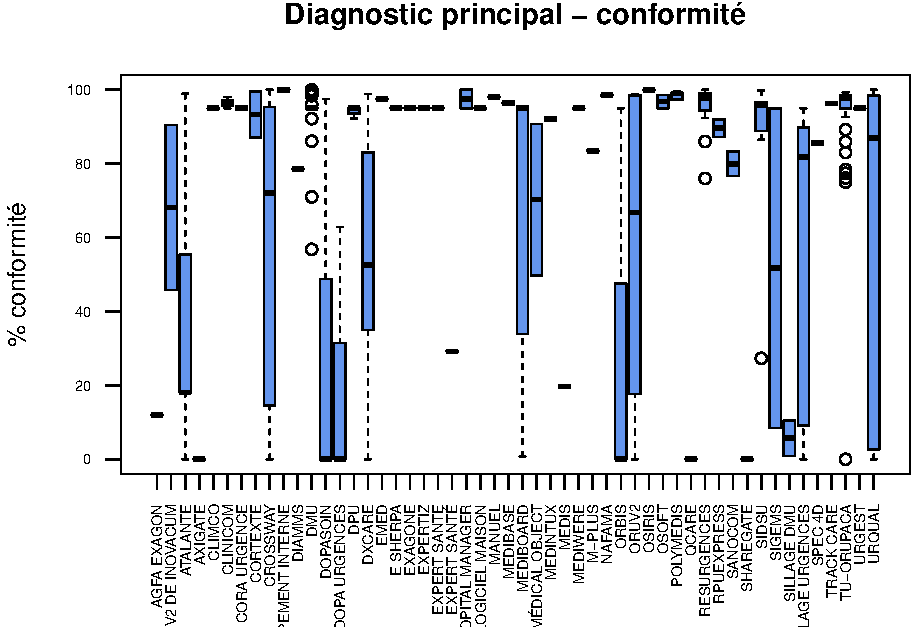
\includegraphics{septembre2015_files/figure-latex/unnamed-chunk-18-1.pdf}

\begin{itemize}
\tightlist
\item
  taux de exhaustivité:
\end{itemize}

\begin{verbatim}
   Min. 1st Qu.  Median    Mean 3rd Qu.    Max.    NA's 
   0.00   43.20   93.10   70.92   98.40  100.00       6 
\end{verbatim}

\begin{itemize}
\tightlist
\item
  exhaustivité par outil
\end{itemize}

\begin{verbatim}
                          Min    Max   moyenne  ecart-type Nb
AGFA EXAGON             12.00  12.00  12.00000          NA  1
ANTARES V2 DE INOVACUM  45.84  90.51  68.17500 31.58645992  2
ATALANTE                 0.00  98.95  38.23222 35.61581102  9
AXIGATE                  0.00   0.00   0.00000          NA  1
CLINICOM                96.14  98.03  97.08500  1.33643182  2
CORTEXTE                87.57  99.52  93.54500  8.44992604  2
CROSSWAY                 0.00 100.00  54.81909 42.91168360 12
DEVELOPPEMENT INTERNE  100.00 100.00 100.00000          NA  1
DIAMMS                  78.72  78.72  78.72000          NA  1
DMU                     56.90 100.00  91.40923 13.08995446 14
DOPA URGENCES            0.00  62.90  20.96667 36.31533193  3
DOPASOIN                 0.00  97.71  32.57000 56.41289480  3
DPU                     92.18  92.18  92.18000          NA  1
DXCARE                   0.00  98.90  54.74923 35.50656429 13
EMED                    97.60  97.60  97.60000          NA  1
EXPERT SANTÉ            29.22  29.22  29.22000          NA  1
HOPITAL MANAGER         95.00 100.00  97.50000  3.53553391  2
M-PLUS                  83.50  83.50  83.50000          NA  1
MANUEL                  99.00  99.00  99.00000          NA  1
MEDIBASE                96.40  96.40  96.40000          NA  1
MEDIBOARD                0.73  43.20  27.90250 20.15014702  4
MÉDICAL OBJECT          49.76  90.77  70.26500 28.99844910  2
MEDINTUX               100.00 100.00 100.00000          NA  1
MEDIS                   19.70  19.70  19.70000  0.00000000  2
NAFAMA                  99.80  99.80  99.80000          NA  1
ORBIS                    0.00   0.00   0.00000  0.00000000  3
ORUV2                    0.00  98.90  58.18500 48.93563017  4
OSIRIS                 100.00 100.00 100.00000          NA  1
OSOFT                   98.60  98.60  98.60000  0.00000000  2
POLYMEDIS               97.40  99.70  98.74000  0.84734881  5
QCARE                    0.00   0.00   0.00000          NA  1
RESURGENCES             76.00 100.00  96.08077  5.00124378 27
RPUEXPRESS              87.22  91.95  89.58500  3.34461508  2
SANOCOM                 76.70  83.30  80.00000  4.66690476  2
SHAREGATE                0.00   0.10   0.05000  0.07071068  2
SIDSU                   27.30  99.80  87.05556 22.82515669  9
SIGEMS                   8.40   8.40   8.40000          NA  2
SILLAGE DMU              0.90  10.50   5.70000  5.54256258  4
SILLAGE URGENCES         0.00  95.00  53.52857 43.21147334 14
SPEC 4D                 85.57  85.57  85.57000          NA  1
TRACK CARE              96.30  96.30  96.30000          NA  1
TU-ORUPACA               0.00  99.29  92.83622 15.63379909 45
URQUAL                   0.00 100.00  62.41706 41.23425066 36
\end{verbatim}

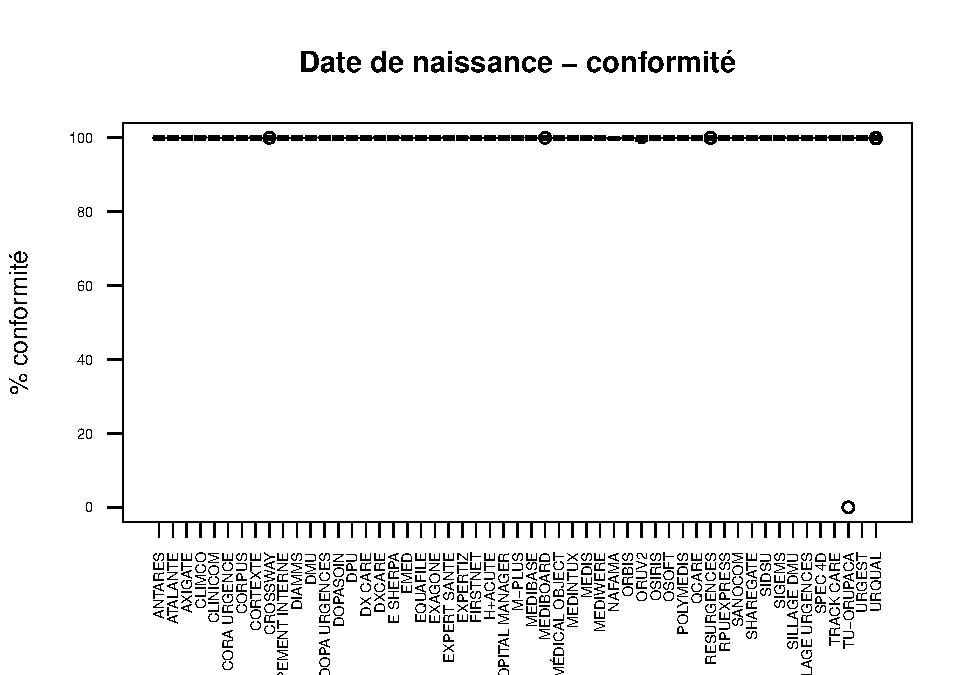
\includegraphics{septembre2015_files/figure-latex/unnamed-chunk-20-1.pdf}

\subsection{Mode de sortie (MS)}\label{mode-de-sortie-ms}

\begin{itemize}
\tightlist
\item
  taux de conformité:
\end{itemize}

\begin{verbatim}
Warning: NAs introduits lors de la conversion automatique
\end{verbatim}

\begin{verbatim}
   Min. 1st Qu.  Median    Mean 3rd Qu.    Max.    NA's 
   0.00   93.88   99.50   87.70   99.99  100.00       5 
\end{verbatim}

\begin{itemize}
\tightlist
\item
  conformité par outil
\end{itemize}

\begin{verbatim}
                          Min    Max   moyenne ecart-type Nb
AGFA EXAGON            100.00 100.00 100.00000         NA  1
ANTARES V2 DE INOVACUM  83.99  84.48  84.23500  0.3464823  2
ATALANTE                 0.00  99.14  59.77889 37.0790394  9
AXIGATE                 99.90  99.90  99.90000         NA  1
CLINICOM                98.66 100.00  99.33000  0.9475231  2
CORTEXTE                99.43  99.70  99.56500  0.1909188  2
CROSSWAY                 0.00  99.44  49.59364 47.9639632 12
DEVELOPPEMENT INTERNE   99.89  99.89  99.89000         NA  1
DIAMMS                  80.47  80.47  80.47000         NA  1
DMU                     97.41 100.00  99.39071  1.0119096 14
DOPA URGENCES           69.10  82.60  77.36667  7.2431577  3
DOPASOIN                72.48  86.54  78.59333  7.2070614  3
DPU                     99.76  99.76  99.76000         NA  1
DXCARE                  21.05 100.00  86.82538 29.3565517 13
EMED                   100.00 100.00 100.00000         NA  1
EXPERT SANTÉ            99.93  99.93  99.93000         NA  1
HOPITAL MANAGER        100.00 100.00 100.00000  0.0000000  2
M-PLUS                  16.80  16.80  16.80000         NA  1
MANUEL                  99.00  99.00  99.00000         NA  1
MEDIBASE                65.70  65.70  65.70000         NA  1
MEDIBOARD               99.53  99.96  99.85000  0.2133854  4
MÉDICAL OBJECT          49.52  90.67  70.09500 29.0974440  2
MEDINTUX               100.00 100.00 100.00000         NA  1
MEDIS                   13.50  13.50  13.50000  0.0000000  2
NAFAMA                  99.80  99.80  99.80000         NA  1
ORBIS                   15.70  19.80  18.43333  2.3671361  3
ORUV2                   39.45  99.92  84.27000 29.8845211  4
OSIRIS                 100.00 100.00 100.00000         NA  1
OSOFT                  100.00 100.00 100.00000  0.0000000  2
POLYMEDIS               99.30  99.90  99.68000  0.2683282  5
QCARE                    0.00   0.00   0.00000         NA  1
RESURGENCES              0.00 100.00  87.95385 32.4504998 27
RPUEXPRESS              93.58  94.01  93.79500  0.3040559  2
SANOCOM                100.00 100.00 100.00000  0.0000000  2
SHAREGATE              100.00 100.00 100.00000  0.0000000  2
SIDSU                   98.20 100.00  99.45556  0.5659309  9
SIGEMS                  99.90  99.90  99.90000         NA  2
SILLAGE DMU             98.80 100.00  99.40000  0.6928203  4
SILLAGE URGENCES        68.50  99.90  93.73571 11.0225369 14
SPEC 4D                 99.97  99.97  99.97000         NA  1
TRACK CARE              98.30  98.30  98.30000         NA  1
TU-ORUPACA               0.00 100.00  94.65756 15.6655159 45
URQUAL                  14.29 100.00  93.47882 15.6017943 36
\end{verbatim}

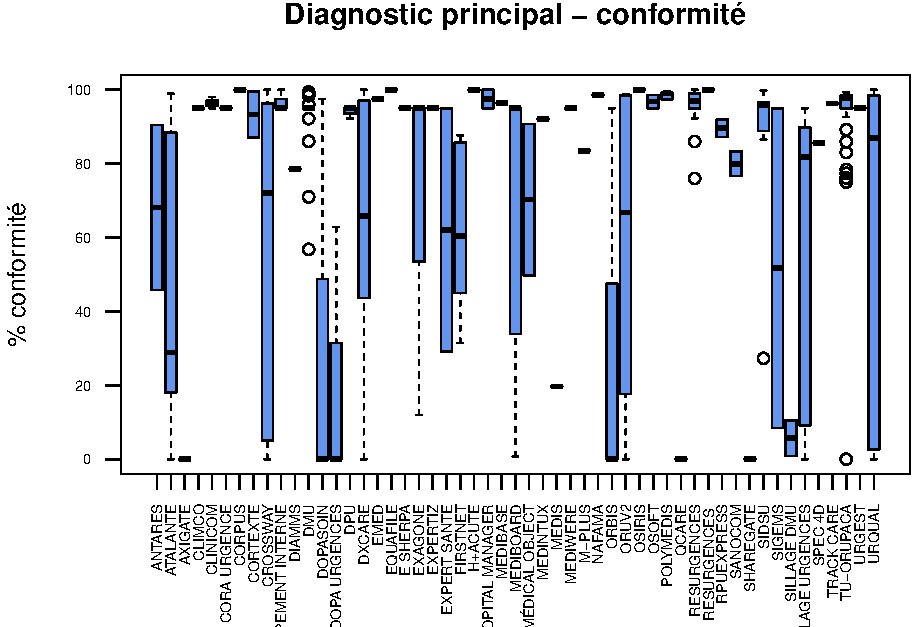
\includegraphics{septembre2015_files/figure-latex/unnamed-chunk-22-1.pdf}

\begin{itemize}
\tightlist
\item
  taux de exhaustivité:
\end{itemize}

\begin{verbatim}
Warning: NAs introduits lors de la conversion automatique
\end{verbatim}

\begin{verbatim}
   Min. 1st Qu.  Median    Mean 3rd Qu.    Max.    NA's 
   0.00   95.10   99.60   88.11  100.00  100.00       5 
\end{verbatim}

\begin{itemize}
\tightlist
\item
  exhaustivité par outil
\end{itemize}

\begin{verbatim}
                          Min    Max   moyenne  ecart-type Nb
AGFA EXAGON            100.00 100.00 100.00000          NA  1
ANTARES V2 DE INOVACUM  83.99  84.48  84.23500  0.34648232  2
ATALANTE                 0.00  99.14  59.77889 37.07903938  9
AXIGATE                100.00 100.00 100.00000          NA  1
CLINICOM                99.92 100.00  99.96000  0.05656854  2
CORTEXTE                99.43  99.70  99.56500  0.19091883  2
CROSSWAY                 0.00  99.44  49.60273 47.97343850 12
DEVELOPPEMENT INTERNE  100.00 100.00 100.00000          NA  1
DIAMMS                  80.47  80.47  80.47000          NA  1
DMU                     97.41 100.00  99.39071  1.01190958 14
DOPA URGENCES           69.10  82.60  77.36667  7.24315769  3
DOPASOIN                72.48 100.00  86.34000 13.76109007  3
DPU                     99.76  99.76  99.76000          NA  1
DXCARE                  21.05 100.00  86.85923 29.37125847 13
EMED                   100.00 100.00 100.00000          NA  1
EXPERT SANTÉ           100.00 100.00 100.00000          NA  1
HOPITAL MANAGER        100.00 100.00 100.00000  0.00000000  2
M-PLUS                  16.80  16.80  16.80000          NA  1
MANUEL                  99.00  99.00  99.00000          NA  1
MEDIBASE                65.70  65.70  65.70000          NA  1
MEDIBOARD               99.53  99.96  99.85000  0.21338541  4
MÉDICAL OBJECT          49.76  90.69  70.22500 28.94188055  2
MEDINTUX               100.00 100.00 100.00000          NA  1
MEDIS                   13.50  13.50  13.50000  0.00000000  2
NAFAMA                  99.80  99.80  99.80000          NA  1
ORBIS                   15.70  19.80  18.43333  2.36713610  3
ORUV2                   99.04 100.00  99.71000  0.44944410  4
OSIRIS                 100.00 100.00 100.00000          NA  1
OSOFT                  100.00 100.00 100.00000  0.00000000  2
POLYMEDIS               99.30  99.90  99.68000  0.26832816  5
QCARE                    0.00   0.00   0.00000          NA  1
RESURGENCES              0.00 100.00  87.95385 32.45049979 27
RPUEXPRESS              98.37  99.94  99.15500  1.11015765  2
SANOCOM                100.00 100.00 100.00000  0.00000000  2
SHAREGATE              100.00 100.00 100.00000  0.00000000  2
SIDSU                   98.20 100.00  99.45556  0.56593089  9
SIGEMS                  99.90  99.90  99.90000          NA  2
SILLAGE DMU             98.80 100.00  99.40000  0.69282032  4
SILLAGE URGENCES        68.50  99.90  93.73571 11.02253685 14
SPEC 4D                 99.97  99.97  99.97000          NA  1
TRACK CARE              98.30  98.30  98.30000          NA  1
TU-ORUPACA               0.00 100.00  94.65756 15.66551586 45
URQUAL                  14.29 100.00  93.47882 15.60179433 36
\end{verbatim}

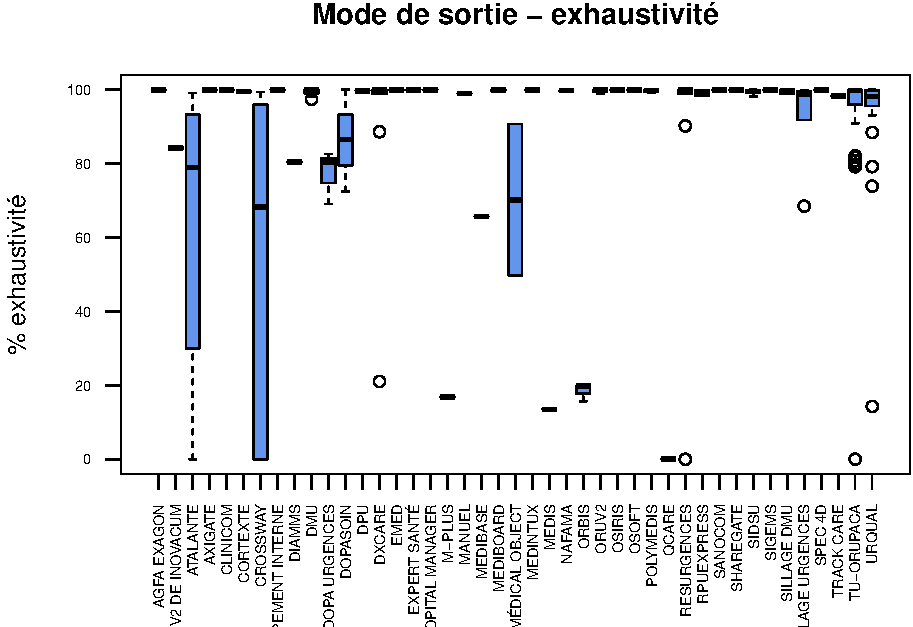
\includegraphics{septembre2015_files/figure-latex/unnamed-chunk-24-1.pdf}

\section{Conformité par région}\label{conformite-par-region}

\subsection{Date de naissance}\label{date-de-naissance-1}

\begin{verbatim}
                      Min Max   moyenne  ecart-type Nb
ALSACE             100.00 100 100.00000  0.00000000 18
AQUITAINE          100.00 100 100.00000  0.00000000 35
BOURGOGNE          100.00 100 100.00000  0.00000000 23
BRETAGNE            99.80 100  99.99077  0.03904980 55
CHAMPAGNE ARDENNES  99.80 100  99.98750  0.05000000 16
LIMOUSIN            99.95 100  99.99333  0.01658312  9
MIDI PYRENEES       98.74 100  99.95054  0.20698827 37
PACA                 0.00 100  97.99800 14.14185177 50
\end{verbatim}

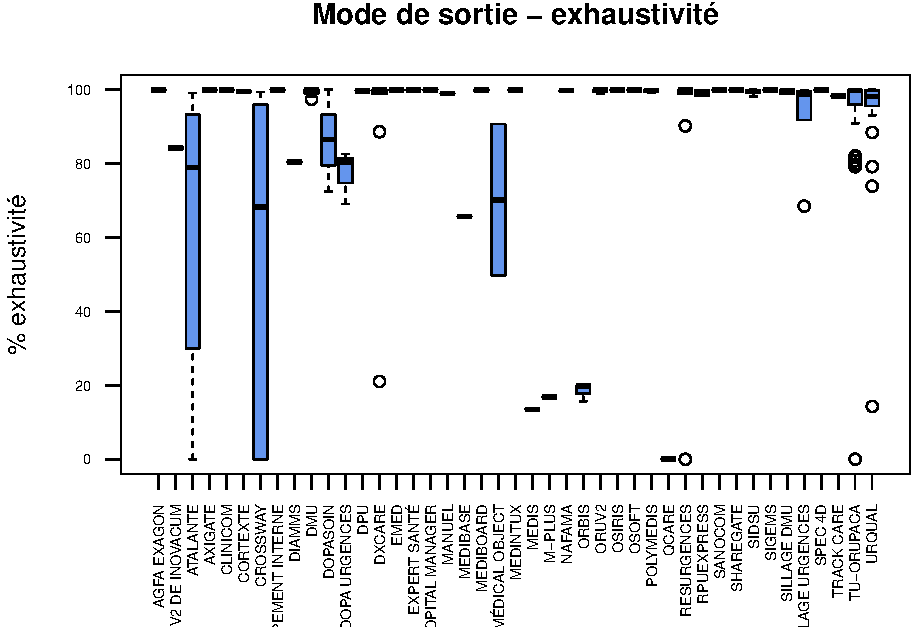
\includegraphics{septembre2015_files/figure-latex/unnamed-chunk-25-1.pdf}

\subsection{Diagnostic (DP)}\label{diagnostic-dp-1}

\begin{verbatim}
                     Min    Max  moyenne ecart-type Nb
ALSACE              0.00  98.95 50.13176  34.316355 18
AQUITAINE           0.00  99.80 63.42121  39.782563 35
BOURGOGNE           0.00 100.00 63.86957  44.685064 23
BRETAGNE            0.00 100.00 61.07250  40.936960 55
CHAMPAGNE ARDENNES  0.00  99.70 67.61875  41.100790 16
LIMOUSIN           85.57  98.98 96.81667   4.256727  9
MIDI PYRENEES       0.00 100.00 70.32676  37.940900 37
PACA                0.00  99.39 88.78780  23.584018 50
\end{verbatim}

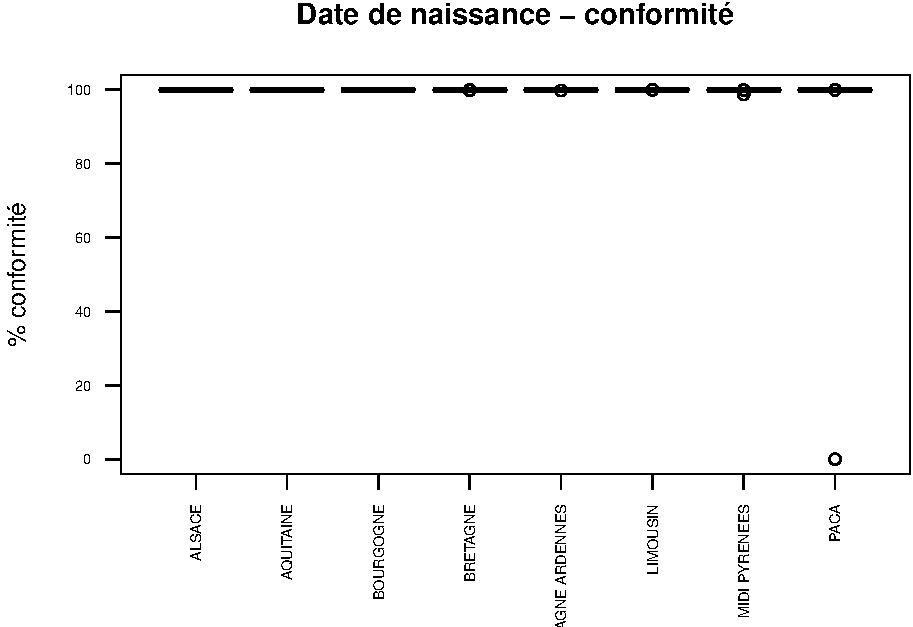
\includegraphics{septembre2015_files/figure-latex/unnamed-chunk-26-1.pdf}

\subsection{Mode de sortie (MS)}\label{mode-de-sortie-ms-1}

\begin{verbatim}
                     Min Max  moyenne ecart-type Nb
ALSACE             15.70 100 68.77500 32.8245757 18
AQUITAINE           0.00 100 89.24242 27.5958220 35
BOURGOGNE           0.00 100 82.04348 38.5091232 23
BRETAGNE           13.50 100 90.35038 22.8208664 55
CHAMPAGNE ARDENNES 69.10 100 94.84375  9.6193533 16
LIMOUSIN           99.39 100 99.88667  0.2200568  9
MIDI PYRENEES       0.00 100 89.86405 20.8648135 37
PACA                0.00 100 87.24620 29.0773015 50
\end{verbatim}

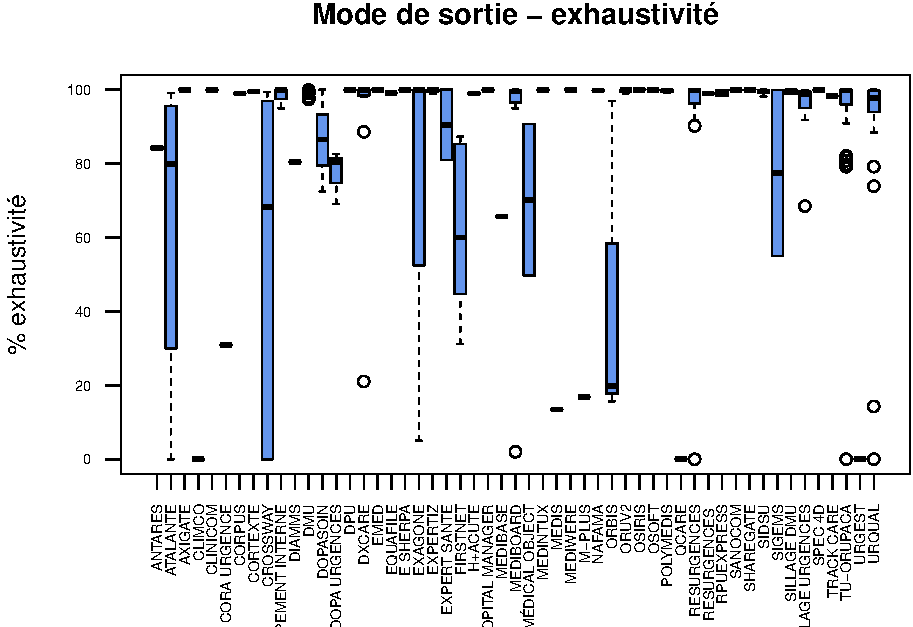
\includegraphics{septembre2015_files/figure-latex/unnamed-chunk-27-1.pdf}

\section{Exhaustivié par région}\label{exhaustivie-par-region}

\subsection{Date de naissance}\label{date-de-naissance-2}

\begin{verbatim}
                      Min Max   moyenne  ecart-type Nb
ALSACE             100.00 100 100.00000  0.00000000 18
AQUITAINE          100.00 100 100.00000  0.00000000 35
BOURGOGNE          100.00 100 100.00000  0.00000000 23
BRETAGNE           100.00 100 100.00000  0.00000000 55
CHAMPAGNE ARDENNES  99.80 100  99.98750  0.05000000 16
LIMOUSIN            99.95 100  99.99333  0.01658312  9
MIDI PYRENEES       99.96 100  99.99676  0.01028863 37
PACA                 0.00 100  97.99800 14.14185177 50
\end{verbatim}

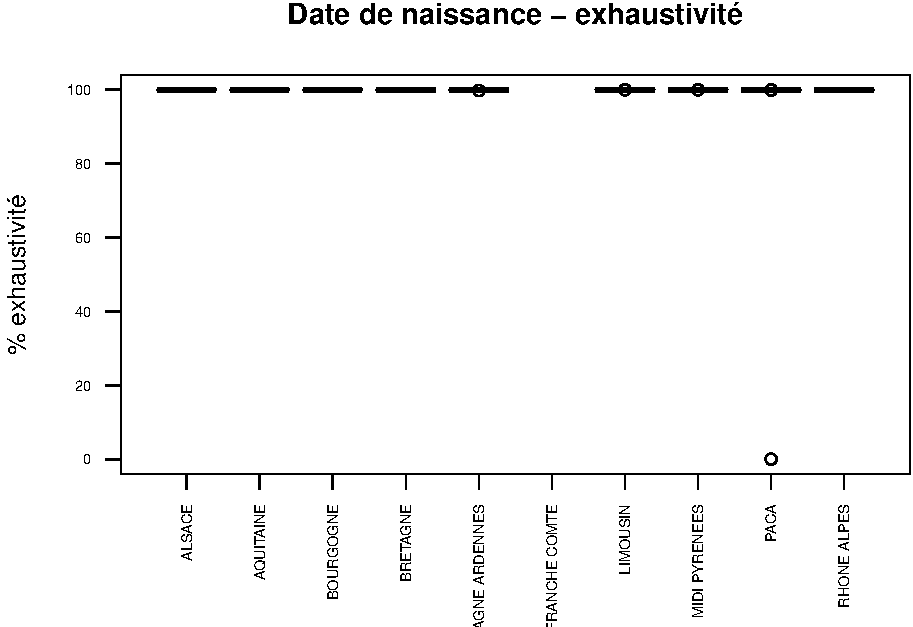
\includegraphics{septembre2015_files/figure-latex/unnamed-chunk-28-1.pdf}

\subsection{Diagnostic (DP)}\label{diagnostic-dp-2}

\begin{verbatim}
                     Min    Max  moyenne ecart-type Nb
ALSACE              0.00  98.95 50.13176  34.316355 18
AQUITAINE           0.00  99.80 63.42424  39.784993 35
BOURGOGNE           0.00 100.00 63.91304  44.720255 23
BRETAGNE            0.00 100.00 62.72885  40.153125 55
CHAMPAGNE ARDENNES  0.00  99.80 74.30625  37.783161 16
LIMOUSIN           85.57  98.98 96.81667   4.256727  9
MIDI PYRENEES       0.00 100.00 70.79919  38.082150 37
PACA                0.00 100.00 89.00340  23.627537 50
\end{verbatim}

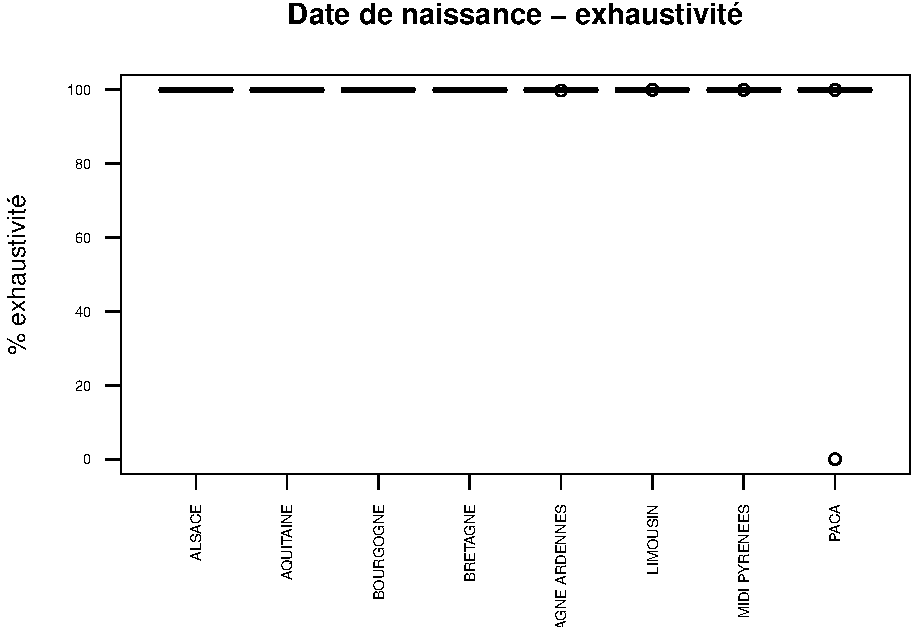
\includegraphics{septembre2015_files/figure-latex/unnamed-chunk-29-1.pdf}

\subsection{Mode de sortie (MS)}\label{mode-de-sortie-ms-2}

\begin{verbatim}
                     Min Max  moyenne ecart-type Nb
ALSACE             15.70 100 68.77500 32.8245757 18
AQUITAINE           0.00 100 89.24848 27.5976915 35
BOURGOGNE           0.00 100 82.04348 38.5091232 23
BRETAGNE           13.50 100 90.35038 22.8208664 55
CHAMPAGNE ARDENNES 69.10 100 94.84375  9.6193533 16
LIMOUSIN           99.39 100 99.88667  0.2200568  9
MIDI PYRENEES       0.00 100 92.50892 19.0664729 37
PACA                0.00 100 87.24620 29.0773015 50
\end{verbatim}

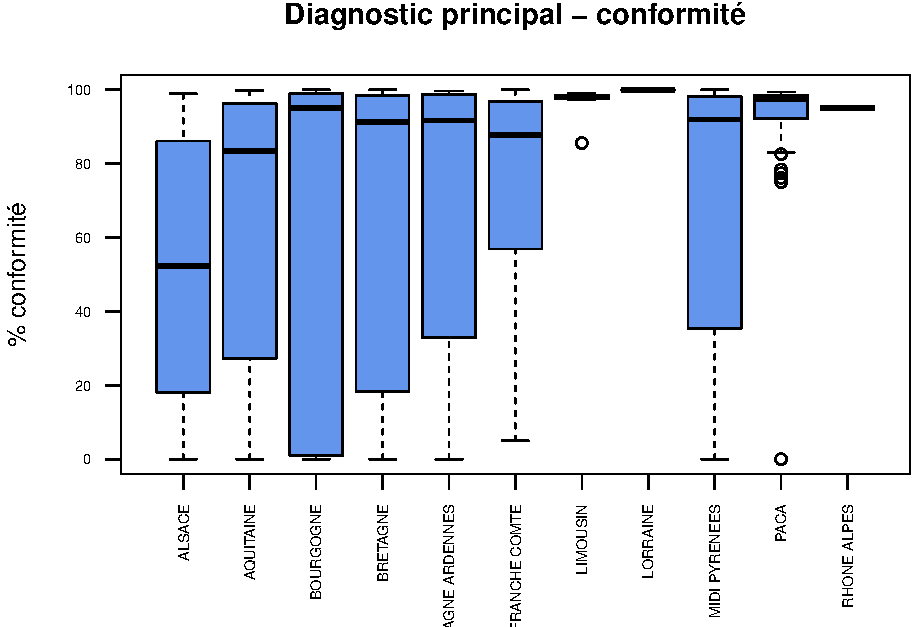
\includegraphics{septembre2015_files/figure-latex/unnamed-chunk-30-1.pdf}

\section{Résultats secondaires}\label{resultats-secondaires}

\subsection{\% de SU ne faisant pas de remontée de
RPU}\label{de-su-ne-faisant-pas-de-remontee-de-rpu}

\begin{verbatim}

 NON  OUI OUI  
  17  225    1 
\end{verbatim}

\begin{verbatim}
[1] "7 %"     "92.59 %" "0.41 %" 
\end{verbatim}

Messges pour les éditeurs, la DGOS, les DSI qui est responsable de quoi
? intégratin systématique des thésaurus, démarche d'amélioration.
Information proactive des sociétés savantes pour la publicationn des
Référentiels: info systématique de la Fedoru. Focaliser sur les
rectangles bleus. Voir si le n° de version permet de discriminer les
urqual qui remntent de ceux qui remontent mal.

\end{document}
